 %%%%%%%%%%%%%%%%%%%%%%%%%%%%%%%%%%%%%%%%%%%%%%%%
%%%%%%%%%%%%%%%%%%%%%%%%%%%%%%%%%%%%%%%%%%%%%%%%
\documentclass[10pt]{article}

%%%%%%%%%%%%%%%%%%%%%%%%%%%%%%%%%%%%%%%%%%%%%%%%
% Package UPSTI_Document
%%%%%%%%%%%%%%%%%%%%%%%%%%%%%%%%%%%%%%%%%%%%%%%% 
\RequirePackage{UPSTI_Document}
\usepackage{hyperref}
\hypersetup{
    colorlinks=true,
    linkcolor=black,
%    filecolor=blue,      
    urlcolor=blue,
}
\urlstyle{same}
%\usepackage{pythontex}

\usepackage{graphicx}
\graphicspath{{images/}}
% \newcommand{\executeiffilenewer}[3]{%
% \ifnum\pdfstrcmp{\pdffilemoddate{#1}}%
% {\pdffilemoddate{#2}}>0%
% {\immediate\write18{#3}}\fi%
% }
% \newcommand{\includesvg}[1]{%
% \executeiffilenewer{#1.svg}{#1.pdf}%
% {inkscape --export-area-page --export-dpi=300 --export-type=pdf --export-latex #1.svg}%
% \input{#1.pdf_tex}%
% }

% \usetikzlibrary{circuits.logic.IEC} 
%\renewcommand{\labelitemi}{-}

%---------------------------------%
% Paramètres du package
%---------------------------------%

% Variante
% ------------------------------------------------------
% Permet de changer la mise en forme pour l'adapter à un autre lycée ou une autre classe (voir UPSTI_Custom.sty). Mise en forme par défaut si la ligne reste en commentaire, ou modifiée selon le chiffre passé en paramètre.
% ------------------------------------------------------
%\newcommand{\UPSTIvariante}{3}

% Choix du type de document
% ------------------------------------------------------
% 1: Cours				% 8: Fiche Synthèse
% 2: TD					% 9: Formulaire
% 3: TP					% 10: Mémo
% 4: Colle					% 11: Dossier technique
% 5: DS					% 12: Dossier ressource
% 6: DM					% 13: Concours blanc
% 7: Fiche Méthode			% 14 : Fiche Séquence
% ------------------------------------------------------
\newcommand{\UPSTIidTypeDocument}{2}

% Version du document (pour la compilation)
% ------------------------------------------------------
% 1: Document prof
% 2: Document élève
% 3: Document à publier
% ------------------------------------------------------
\newcommand{\UPSTIidVersionDocument}{1}

% Classe
% ------------------------------------------------------
% 1- TSI1		% 6- MP
% 2- TSI2		% 7- PC
% 3- MPSI	% 8- PSI
% 4- PCSI		% 9- PT
% 5- PTSI
% ------------------------------------------------------
\newcommand{\UPSTIidClasse}{1}

% Matière
% ------------------------------------------------------
% 1: S2I
% 2: IPT
% ------------------------------------------------------
\newcommand{\UPSTIidMatiere}{1}

% Titre du document (dans l'en-tête)
% ------------------------------------------------------
\newcommand{\UPSTInumeroSequence}{11}
\newcommand{\UPSTItitreEnTete}{Déterminer les performances globales d'un système}      
%\newcommand{\UPSTItitreEnTetePages}{Titre pour les en tetes des pages > page 1}      

% Titre principal 
% "Colle: UPSTItitreEnTete \\ UPSTItitre"   ou bien   "UPSTItitrePreambule \\ UPSTItitre")
% ------------------------------------------------------
%\newcommand{\UPSTItitreEnTete}{Analyse système}
\newcommand{\UPSTItitrePreambule}{Asservissement d'altitude d'un drone de surveillance}      
%\newcommand{\UPSTItitre}{Titre}      

% Durée de l'activité (pour DS, DM et TP)
% ------------------------------------------------------
\newcommand{\UPSTIduree}{} 

% Numéro (ajoute " n°1" après DS ou DM)
% ------------------------------------------------------
\newcommand{\UPSTInumero}{07}

% Message sous le titre
% ------------------------------------------------------
%\newcommand{\UPSTImessage}{Message sous le titre}

% Référence au programme
% ------------------------------------------------------
\newcommand{\UPSTIprogramme}{S11 - Validation des performances fréquentielles}

% Source ou inspiration
% ------------------------------------------------------
\newcommand{\UPSTIsource}{Mines-Ponts PSI 2010}
%source : https://www.technologuepro.com/cours-systemes-embarques/cours-systemes-embarques-Bus-CAN.htm

% Note de bas de première page
% ------------------------------------------------------
\newcommand{\UPSTInoteBasDePremierePage}{}      

% Si l'auteur n'est pas l'auteur par défaut
% ------------------------------------------------------
%\renewcommand{\UPSTIauteur}{Nom de l'auteur}

% Si le document est réalisé au nom de l'équipe
% ------------------------------------------------------
%\newcommand{\UPSTIdocumentCollegial}{1}

% Versioning
% ------------------------------------------------------
\newcommand{\UPSTInumeroVersion}{1}
\renewcommand{\UPSTIfooterLycee}{ M.-F. SOULÉ DE LAFONT}
%----------------------------------------------- 
\UPSTIcompileVars		% "Compile" les variables



%%%%%%%%%%%%%%%%%%%%%%%%%%%%%%%%%%%%%%%%%%%%%%%% 
%\DeclareUnicodeCharacter{0301}{\'{e}}

%%%%%%%%%%%%%%%%%%%%%%%%%%%%%%%%%%%%%%%%%%%%%%%% 
% DEBUT DU DOCUMENT
%%%%%%%%%%%%%%%%%%%%%%%%%%%%%%%%%%%%%%%%%%%%%%%% 
\begin{document}

% Création de l'en-tête
\UPSTIbuildPage

%\vspace{-35pt}
%\begin{center}
%\UPSTIdiagrammeCompetences[0.75][2][1][0][0][1][0][0][1]
%\end{center}

%\vspace{-1.5cm}
%\renewcommand{\baselinestretch}{0.75}
%{\scriptsize{\tableofcontents}}
%\renewcommand{\baselinestretch}{1.0}\normalsize
%\input{competences.tex}

\vspace{.5cm}
\UPSTIobjectif{
\small
\begin{itemize}
\item Tracer un diagramme de Bode asymptotique
\item Valider un cahier des charges en précision, amortissement et stabilité 
\end{itemize}
}

\begin{figure}[h!]
\centering
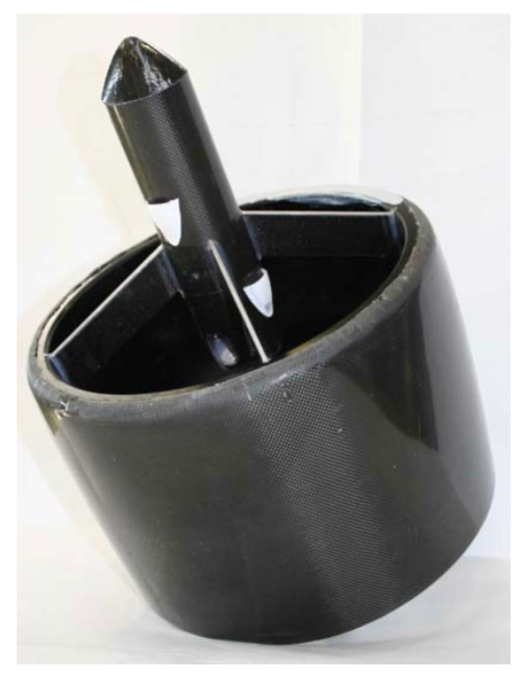
\includegraphics[width=0.25\textwidth]{drone1.pdf}
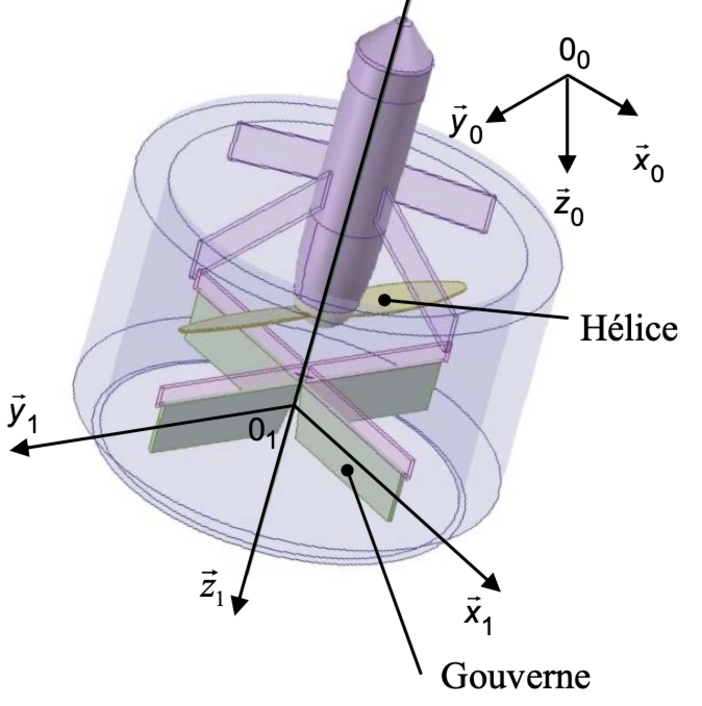
\includegraphics[width=0.25\textwidth]{drone2.pdf}
\caption{Drone à voilure tournante}
\label{drone}
\end{figure}

Le drone Munin est un petit drone volant développé par la Sagem, dédié à la surveillance extérieure de bâtiments ou de zones industrielles. Il parcourt régulièrement une trajectoire préprogrammée et transmet un flux vidéo des zones surveillées. Un opérateur peut redéfinir à tout moment la trajectoire en cas de problème sur une zone, voire rester en vol stationnaire au-dessus
d'une position. Le drone est constitué d'un châssis, d'un moteur fixe sur le châssis entrainant une hélice à
pas fixe et de gouvernes orientables. L'ensemble est commandé par une carte de commande
numérique dialoguant avec le poste de contrôle. La stabilisation est assurée par une centrale inertielle (accéléromètres et gyromètres), un capteur ultra-son mesurant la distance au sol, un capteur barométrique mesurant l'altitude, un capteur GPS mesurant la position géographique. L'objectif de l'étude est de déterminer les lois de commande à implanter dans la carte de commande numérique de façon à assurer des performances correctes du drone. Seule la stabilisation en altitude est envisagée. Le cahier des charges concernant l'asservissement d'altitude est le
suivant :
\begin{itemize}
	\item  Stabilité : \(M G>10 \mathrm{dB}\) et \(M \varphi>60^{\circ}\)
	\item Rapidité : bande passante à -3 dB supérieure à 10 Hz.
\end{itemize}

 La chaine d'action de l'asservissement d'altitude comporte essentiellement un moteur électrique alimenté par un hacheur et entrainant une hélice. La poussée de l'hélice \(F_{h}\) est directement proportionnelle à sa vitesse de rotation \(\omega_{m}\), et conduit à une accélération verticale du drone. La chaine de mesure est constituée des capteurs ultra-son et barométriques, dont les mesure combinées donnent une information d'altitude \(Z\) du drone.

\begin{figure}
\begin{tikzpicture}
	\sbEntree{U}
\sbBoucleRetour[4]{U}{C/$K_p$,A/$K_A$,H/$\dfrac{K_m}{1+\tau_m p}$,kh/$K_h$,mp2/$\dfrac{1}{mp^2}$}{G/$1$}
\node[above of=CompU-C,node distance=0.5em]{$\varepsilon(p)$};
\node[above of=A-H, node distance=0.5em]{$U(p)$};
\node[above of=U,node distance=0.5em]{$Z_c(p)$};
\node[above of=H-kh,node distance=0.5em]{$\Omega_m(p)$};
\node[above of=kh-mp2,node distance=0.5em]{$F_h$};
\sbSortie[7]{V2}{mp2}\sbRelier[$Z(p)$]{mp2}{V2}
\node[above of =C, node distance=-2em]{Correcteur};
\node[above of =A, node distance=-2em]{Hacheur};
\node[above of =H, node distance=-2em]{Moteur};
\node[above of =kh, node distance=-2em]{Hélice};
\node[above of =mp2, node distance=-2em]{Drone};
\node[above of =G, node distance=-2em]{Capteur altitude};
\end{tikzpicture}
\caption{Schéma-blocs de l'asservissement simple de l'altitude du drone}
\label{sb1}
\end{figure}


Le schéma-blocs modélisant l'asservissement est donné \UPSTIfig{sb1}. Le moteur est modélisé par une fonction de transfert du premier ordre de constante de temps \(\tau_{m}=0,2\) s. Les capteurs son supposés renvoyer une information exacte et rapide et leur fonction de transfert est assimilée à u gain unitaire. Les constantes suivantes sont données : \(K_{A}=47 \times 10^{-3} \mathrm{V}\) inc \(^{-1}, K_{m}=25 \mathrm{rad} \mathrm{s}^{-1} \mathrm{V}^{-}\)
\(K_{h}=33 \times 10^{-3} \mathrm{N} \operatorname{srad}^{-1}\) et \(m=1 \mathrm{kg}\).


\UPSTIquestion{Déterminer la fonction de transfert en boucle ouverte \(\mathrm{FTBO}(p)\) de l'asservissement d'altitude du drone.} \label{FTBOalt}

\UPSTIcorrection{
 La fonction de transfert en boucle ouverte pour la première architecture (à une seule boucle) s'écrit :
\[
\mathrm{FTBO}_{1}(p)=K_{p} K_{A} \frac{K_{m}}{1+\tau p} K_{h} \frac{1}{m p^{2}
}
\]
}


\UPSTIquestion{Dessiner l'allure du diagramme de Bode de cette FTBO pour un gain \(K_{p}\) unitaire et préciser les caractéristiques de stabilité à partir de l'étude des marges de gain et de phase. Dans quelle mesure le gain du correcteur peut-il améliorer la stabilité? }\label{FTBO-bode}

\begin{figure}
\centering
\begin{tikzpicture}[xscale=15/3]
\begin{scope}[yscale=6/170]
\UnitedB
\OrdBode{20}
\semilog{-1}{2}{-140}{20}
\end{scope}
\begin{scope}[yshift=-6cm,yscale=6/270]
\UniteDegre
\OrdBode{45}
\semilog{-1}{2}{-270}{0}
\end{scope}
\end{tikzpicture}
\caption{Diagramme de Bode à compléter de la question \ref{FTBO-bode}}
\end{figure}


\UPSTIcorrection{
L'allure du diagramme de Bode est donné figure \UPSTIfig{FTBOsimp}. La phase étant toujours inférieure à \(-180^{\circ},\) le système est nécessairement instable. Une double intégration conduit toujours à cette observation. La constante \(K_{p}\) ne modifie pas la phase donc une correction proportionnelle ne peut pas restabiliser le système, quelle que soit la valeur.

% \begin{figure}[h!]
% \centering
% \includesvg{images/FTBO_simple_Bode_asymp}
% \caption{Réponse à la question \ref{FTBO-bode}: FTBO(p) simple de l'asservissement en altitude}
% \label{FTBOsimp}
% \end{figure}

}

Une seconde architecture de l'asservissement est proposée. À partir des informations des capteurs ultra-son, barométrique et accélérométrique, une information de vitesse est calculée. Un asservissement de vitesse est alors inclus dans la boucle d'asservissement d'altitude tel que sur le schéma-blocs de la \UPSTIfig{sb2}.

\begin{figure}[h!]
\centering
\includegraphics[width=0.8\textwidth]{sb2.pdf}
\caption{Schéma-bloc de l'asservissement avec la boucle en vitesse de l'altitude du drone }
\label{sb2}
\end{figure}


Après avoir réglé le correcteur \(K_{2}\) et vérifié les performances de la boucle de vitesse, le correcteur
\(K_{1}\) sera dimensionné pour valider le cahier des charges.

\UPSTIquestion{Déterminer la fonction de transfert en boucle ouverte \(\mathrm{FTBO}_{\nu}(p)=\frac{V(p)}{\varepsilon_{2}(p)}\) de l'asservissement de vitesse et tracer l'allure du diagramme de Bode. Pour simplifier les notations, on pose : $K_{\nu}=\dfrac{K_{A} K_{m} K_{h}}{m}$.} \label{FTBOv-bode}

\begin{figure}[h!]
\centering
\begin{tikzpicture}[xscale=15/3]
\begin{scope}[yscale=6/100]
\UnitedB
\OrdBode{20}
\semilog{-1}{2}{-100}{0}
\end{scope}
\begin{scope}[yshift=-7cm,yscale=6/180]
\UniteDegre
\OrdBode{45}
\semilog{-1}{2}{-180}{0}
\end{scope}
\end{tikzpicture}
\caption{Diagramme de Bode à compléter de la question \ref{FTBOv-bode}}
\end{figure}





 \UPSTIcorrection{
La fonction de transfert en boucle ouverte pour la boucle de vitesse s'écrit :

% \[ \mathrm{FTBO}_{v}(p)=\) \(\frac{K_{2} K_{1} K_{m} K_{h}}{m p(1+\tau p)} \]
L'allure du diagramme de Bode est donné \UPSTIfig{FTBOvitF}.

% \begin{figure}[h!]
% \centering
% \includesvg{images/FTBO_vitesse_Bode_asymp}
% \caption{Réponse à la question \ref{FTBOv-bode}: FTBOv(p) de l'asservissement en altitude}
% \label{FTBOvitF}
% \end{figure}

 }


\UPSTIquestion{Déterminer la valeur du correcteur \(K_{2}\) permettant d'assurer une bande passante à \(0 \mathrm{dB}\) de \(\omega_{0 d B}=\frac{1}{\tau} .\) Vérifier que l'asservissement de vitesse est bien stable en déterminant les marges de stabilité. La figure 6.26 présente le diagramme de Bode de la fonction de transfert en boucle ouverte de l'asservissement d'altitude \(\mathrm{FTBO}_{2}(p)=\frac{Z(p)}{\varepsilon_{1}(p)}\) pour une correction \(K_{1}\) unitaire.}

\UPSTIcorrection{
	
La bande passante à \(0 \mathrm{dB}\) est satisfaite si \(\left|\mathrm{FTBO}_{v}\left(\frac{j}{\tau}\right)\right|=1,\) soit:

\[
\frac{K_{2} K_{v}}{\frac{1}{\tau}|1+j|}=1 \Longleftrightarrow K_{2}=\frac{\sqrt{2}}{\tau K_{v}}= \SI{182}{{inc.s.m}^{-1}}
\]
La marge de gain est infinie car la phase n'atteint jamais \(-180^{\circ} .\) Pour la pulsation à \(0 \mathrm{dB}\), le premier ordre est à sa pulsation de cassure, si bien que la phase vaut de façon évidente \(-135^{\circ} .\) La marge de phase vaut donc \(45^{\circ}:\) le système est stable.

}

\UPSTIquestion{Déterminer la fonction de transfert en boucle fermée \(\mathrm{FTBF}_{v}(p)=\frac{V(p)}{V_{c}(p)}\) de l'asservissement de vitesse en précisant les caractéristiques (pulsation propre et amortissement). Justifier alors l'allure du diagramme de Bode proposé \UPSTIfig{FTBO2_Bode} et \UPSTIfig{FTBO2_Black}.}

% \begin{figure}[h!]
% \centering
% \includesvg{images/FTBO2_Bode}
% \caption{Diagramme de Bode de FTBO2(p) de l'asservissement en altitude avec boucle de vitesse avec $K2$ identifié.}
% \label{FTBO2_Bode}
% \end{figure}

% \begin{figure}[h!]
% \centering
% \includesvg{images/FTBO2_Black}
% \caption{Diagramme de Black de FTBO2(p) de l'asservissement en altitude avec boucle de vitesse avec $K2$ identifié.}
% \label{FTBO2_Black}
% \end{figure}


\UPSTIcorrection{
La fonction de transfert en boucle fermée pour la boucle de vitesse $FTBOv(p)$s'écrit, pour la valeur de \(K_{2}\) précédente :

\[\mathrm{FTBF}_{v}(p)=\frac{K_{2} K_{\mu}}{p(1+\tau p)+K_{2} K_{v}}=\frac{1}{\frac{\tau^{2}}{\sqrt{2}} p^{2}+\frac{T}{\sqrt{2}} p+1}\]

Par identification, la pulsation propre vaut \(\omega_{0}=\frac{\sqrt[4]{2}}{\tau}=6 \operatorname{rad} \mathrm{s}^{-1}\) et \(\frac{2 \xi}{\omega_{0}}=\frac{\tau}{\sqrt{2}}\) implique 
\[\xi=\frac{\sqrt[4]{2}}{2\sqrt{2}}\approx 0.42\]

Le diagramme de Bode de la FTBO2(p) est donc la superposition de la fonction de transfert \(\mathrm{FTBF}_{v}(p)\) et d'un intégrateur pur:
\[FTBO2(p)=FTBOv(p)\dfrac{1}{p}\]
Le diagramme proposé montre bien la pente à \(-20 \mathrm{dB} / \mathrm{dec}\) à basse pulsation, puis la pente à \(-60 \mathrm{dB} /\) dec à haute pulsation. L'amortissement est inférieur à \(\frac{\sqrt{2}}{2}\) donc il y a présence d'une légère résonance sur le diagramme de Bode \UPSTIfig{FTBO2_Bode}.
}


\UPSTIquestion{Déterminer sur la courbe \UPSTIfig{FTBO2_Black}, pour un gain \(K_{1}\) unitaire, les marges de stabilités et la bande passante . Cette configuration est-elle satisfaisante au regard des critères du cahier des charges ?}\label{FTBO2_BlackQ}

\UPSTIcorrection{Les marges de gain et de phase sont directement mesurables sur l'abaque de Black \UPSTIfig{FTBO2_Black_margin} : 

% \begin{figure}[h!]
% \centering
% \includesvg{images/FTBO2_Black_margin}
% \caption{Réponse à la question \ref{FTBO2_BlackQ} : Diagramme de Black de FTBO2(p) de l'asservissement en altitude avec boucle de vitesse avec $K_2$ identifié.}
% \label{FTBO2_Black_margin}
% \end{figure}

\(M G=\) \(14 \mathrm{dB}\) et \(M \varphi=82^{\circ} .\) Le système est donc stable et les niveaux de stabilité du cahier des charges sont largement satisfaits. Par contre, la bande passante à \(0 \mathrm{dB}\) sur la FTBO2(p) est voisine de \(1 \mathrm{rad} \mathrm{s}^{-1}\) si bien que la bande passante \(\mathrm{a}-3 \mathrm{dB}\) de la FTBF sera inférieure au niveau exigé par le cahier des charges : le système sera trop lent (temps de réponse de l'ordre de 3 s).}

\UPSTIquestion{Existe-t-il une valeur de \(K_{1}\) permettant de valider le cahier des charges? Le cas échéant déterminer la valeur assurant la meilleure rapidité possible et respectant l'ensemble des
critères.}

\UPSTIcorrection{Pour espérer valider le cahier des charges en terme de bande passante, il faut augmenter la constante \(K_{1}\). Pour obtenir la rapidité maximale, il faut réduire les marges de stabilité au minimum impose par le cahier des charges. La marge de stabilité la plus critique est la marge de gain à \(10 \mathrm{dB}\), qui permet seulement de remonter la courbe de gain de \(4 \mathrm{dB}\), soit

\[ K_{1}=10^{4 / 20}=1,58 \mathrm{s}^{-1} \]
Pour cette valeur de \(K_{1}\), la phase vaut \(-105^{\circ}\) soit une marge de phase de \(75^{\circ}\) ce qui est largement suffisant, et la bande passante vaut 1,65 rad \(s^{-1}=0,26\) Hz.
}

\UPSTIquestion{Comparer la valeur de la bande passante à \(0 \mathrm{dB}\) de la FTBO2(p), la valeur de la bande passante \(-3 \mathrm{dB}\) de la FTBF(p) et la valeur exigée au cahier des charges.}

\UPSTIcorrection{La bande passage est toujours inférieure à celle voulue dans le cahier des charges, il faudrait choisir un autre correcteur pour obtenir les performances souhaitées.}


\end{document}

